%
% conditions.tex --
%
% (c) 2019 Prof Dr Andreas Mueller
%
\section{Boundary conditions\label{klassifikation:randbedingungen}}
\rhead{Boundary conditions}
\index{boundary conditions}
As with ordinary differential equations it is not enough to 
specify the partial differential equation to determine the
solution.
This section shows how the concept of initial conditions and boundary
conditions needs to be extended for partial differential equations.

\subsection{Initial and boundary conditions for ordinary differential equations\label{klassifkation:anfangswerte-ode}}
For ordinary differential equations, we have to specify initial or boundary
conditions.
To fix the differential equation
\[
y''+p(x)y'+q(x)y=0
\]
on the interval
$[0,1]$,
we need two additional conditions, any of the following types of conditions
will do:
\begin{itemize}
\item the values $y(0)$ and $y'(0)$ (initial conditions)
\item the values $y(0)$ und $y(1)$ (boundary conditions)
\item two linear equations combining these
\begin{align*}
\alpha_0y(0)+\beta_0y'(0)&=\gamma_0\\
\alpha_1y(1)+\beta_1y'(1)&=\gamma_1.
\end{align*}
%wobei die Koeffizientenmatrix auf der linken Seite regulär sein muss.
\end{itemize}

\begin{beispiel}
\begin{figure}
\centering
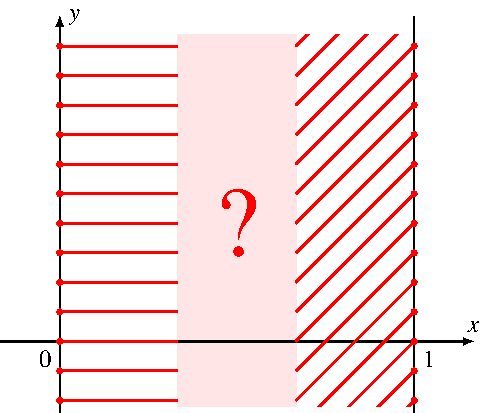
\includegraphics{2-classification/images/mismatch.pdf}
\caption{Specifying derivatives at both ends of the interval for the
differential equation $y''=0$ leads to a contradiction.
The boundary value $y'(0)=0$ means that the solution must be a straight
line with slope $0$, but the boundary value $y'(1)=1$ forces a straight
line with slope $1$.
There is no way to reconcile these conditions.
\label{boundary:mismatch}}
\end{figure}
Even for an linear ordinary differential equation of second order
not every combination of boundary values will allow a solution.
The equation
\[
y''=0
\]
means that the solution curve does not have curvature.
Consequently the solution is a straight line with equation $y=Ax+B$.
In particular, the slope must be equal at both ends of the interval.
The boundary values
\[
y'(0)=0\qquad\text{and}\qquad y'(1)=1,
\]
thus lead to a problem that has no solution (see
figure~\eqref{boundary:mismatch}).
\end{beispiel}

\subsection{Boundary values for partial differential equations\label{klassifikation:randwerte-pde}}
Specifying the boundary values for partial differential equations
becomes much more complicated.
To develop some intuition for this task, let's look again at the
vibrating string.
\begin{figure}
\begin{center}
%\includegraphics{../common/images/randwerte-1.pdf}
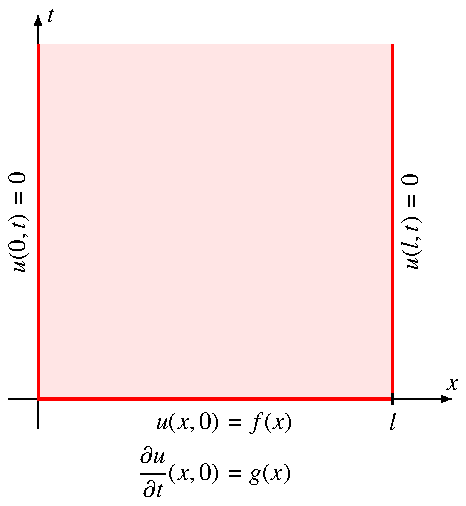
\includegraphics{2-classification/images/wave.pdf}
\end{center}
\caption{boundary values for the wave equation for a vibrating string.
The domain is colored light red, the boundary is red, the boundary
values are specified along the boundary.
\label{klassifikation:randwertesaite}}
\end{figure}
In figure \ref{klassifikation:randwertesaite}
we have drawn the domain in light red.
Boundary values can be given on the left, right and bottom portions
of the boundary.

The theory of ordinary differential equations teaches that a 
differential equation of second order needs precisly two independent
boundary values.
We can either give values at each end of an interval or the value and the
first derivative at one end.

We do the same for the wave equation.
If we forget the $t$ dependence for a moment, we are reduced to a
differential equation of second order in $x$ on the interval $[0,l]$,
so we expect that we can give boundary values at each end
as in
\[
u(0,t)=0\qquad u(l,t)=0.
\]
If we disregard the $x$-dependence, we are left with a differential equation
in $t$ for $t>0$, i.~e.~the only choice for boundary conditions is to
specify the value and the first derivative at $t=0$.

In principle there are multiple first derivatives.
However, if we already know the values of $u(x,0)=f(x)$ along the bottom
boundary, we
also know the values of the first derivative with respect to $x$, it is
\[
\frac{\partial }{\partial x}u(x,0) = f'(x)
\]
We no longer have the option to specify this derivative.
So the only derivative we can reasonably specify on the boundary
is the one with respect to $t$, or in the direction
orthogonal to the boundary.

It turns out that these boundary conditions do in fact uniquely
determine the solution.
Unfortunately this relatively straight forward discussion becomes
much more complicated for general domains.

\subsubsection{General Discussion}
Right from the start we don't even know on which part of the boundary
we should try to specify boundary conditions.
In principle we can use any part of the boundary, but it may happen
that we may not be able to choose boundary values on all of the boundary
freely.
Values on some part of the boundary may already define the values on
other parts of the boundary.

In addition, we have to decide whether to involve derivatives of the
unknown function, which we have already seen cannot be specified
arbitrarily but are subject to certain restrictions, that we would like
to highlight with the following example.
Consider the half plane
\[
\Omega=\{(x,y)\in\mathbb R^2\,|\,x>0\}.
\]
Let $u$ be a function defined on $\bar\Omega$.
If the values of $u$ are given along the boundary $\partial\Omega$
then we also know the derivatives in direction tangential to the boundary:
\[
\text{
$u(0,y)$ known
}\qquad\Rightarrow\qquad
\text{$\frac{\partial u}{\partial y}$ known.}
\]
This we can only reasonably expect to specify derivatives orthogonally
to the boundary.

Consider now the general case: the function $u$ ist defined in a point 
$x=(x_1,\dots,x_k)\in\mathbb R^k$ of the boundary $\partial\Omega$.
We assume that $\partial \Omega$ has a well defined tangential plane
in $x$.
If we know the function values along the boundary, then we know all the
partial derivatives of $u$ in directions tangent to the boundary.
They are computed using the directional derivative
\[
D_{\vec v}u(x_1,\dots,x_k)=\vec v\cdot\operatorname{grad}u
\]
for vectors $\vec{v}$ in the tangent plane.
The only derivative not known yet is the derivative in the direction
orthogonal to the tangent plane.

\begin{definition}
\label{definition:normal-derivative}
Let $\vec{n}$ be the normal vector of a tangent plane of the boundary
of a domain $\Omega$, then the {\em normal derivative}
\index{normal derivative}
is the directional derivative
\[
\frac{\partial u}{\partial n}
=
\frac{\partial u}{\partial \vec{n}}
=
\vec{n}\cdot \operatorname{grad}u .
\]
in the direction of $\vec{n}$
\end{definition}

\begin{beispiel}
Let $\Omega=\{(x,y)\in\mathbb R^2\,|\,x^2+y^2<1\}$ be the unit disk.
Find the normal derivative of the function
$u(x,y)=x^3y$
in each point on the unit circle.

The outside normal in the point $(x,y)$ is
\[
\vec n=\begin{pmatrix}x\\y\end{pmatrix}
\]
\begin{figure}
\centering
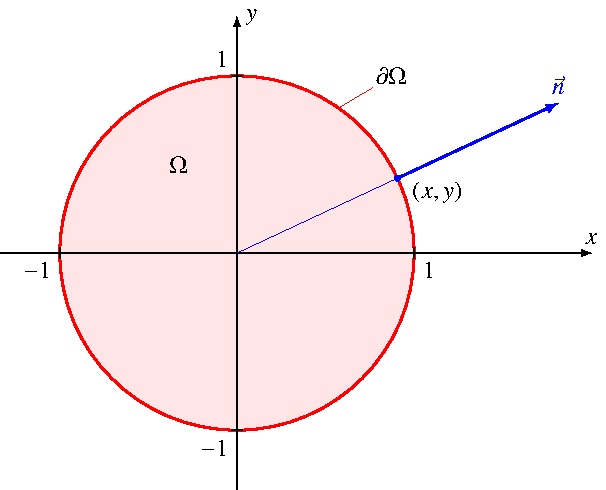
\includegraphics{2-classification/images/disk.pdf}
\caption{Outside normal of disk shaped domain
\label{conditions:outside-normal}}
\end{figure}
(see figure~\ref{conditions:outside-normal}).
The derivative of a function $u(x,y)$
in this direction then is
\[
\frac{\partial u}{\partial n}=
x\frac{\partial u}{\partial x}
+
y\frac{\partial u}{\partial y}.
\]
For the function given in the problem $u(x,y)=x^3y$:
\[
\frac{\partial u}{\partial n}
=
x\cdot 3x^2y+y\cdot x^3=
4x^3y.
\qedhere
\]
\end{beispiel}

\begin{beispiel}
\begin{figure}
\centering
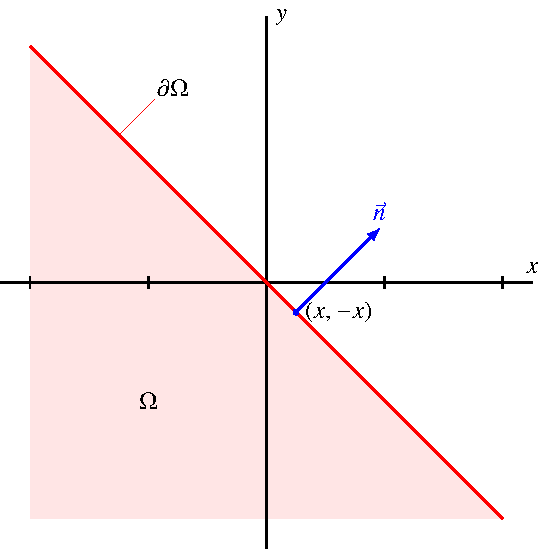
\includegraphics{2-classification/images/oblique.pdf}
\caption{Normal derivative on the boundary of the domain
$\Omega=\{(x,y)\,|\, x+y<0\}$
\label{conditions:oblique}}
\end{figure}
Find the normal derivative of the function
$x^2-y^2$
on the boundary of the domain
$\Omega=\{(x,y)\in\mathbb R^2\,|\,y+x<0\}$
(see figure~\ref{conditions:oblique}).

The domain has the straight line
$y=-x$ as boundary, which has the vector
\[
\vec n=\frac{1}{\sqrt{2}}\begin{pmatrix}1\\1\end{pmatrix}
\]
as its unit normal.
The directional derivative of $u$ in this direction 
in the point $(x,y)$ is
\[
D_{\vec n}u(x,y)
=
\vec n\cdot\operatorname{grad}u
=
\frac{1}{\sqrt{2}}
\begin{pmatrix}1\\1\end{pmatrix}\cdot\begin{pmatrix}2x\\-2y\end{pmatrix}
=
\sqrt{2}( x-y)
\]
In the point $(x,-x)$ on the boundary the normal derivative becomes
\[
\frac{\partial u}{\partial n}
=
\frac{1}{\sqrt{2}}
\frac{\partial u}{\partial x}
+
\frac{1}{\sqrt{2}}
\frac{\partial u}{\partial x}
=
\sqrt{2}(
x+x)
=
2\sqrt{2}x.
\qedhere
\]
\end{beispiel}

\subsection{Particular Cases\label{klassifikation:randwerte-speziell}}
\subsubsection{The Cauchy problem\label{klassifikation:cauchy-problem}}
\index{Cauchy problem}
The boundary of a domain usually consists of many more than just a few
points, usually of curves and surfaces.
To better understand the problem of specifying boundary conditions
we look more closely at the case of a function $u(x,y)$ of two independent
variables.
The solution function $u(x,y)$ can be visualized as a surface over the
$x$-$y$-plane also called the graph of $u$.

The boundary of a domain in $\mathbb R^2$ ist a curve.
If we prescribe values of the function $u(x,y)$ on this curve, we
essentially prescribe a curve contained in the graph of $u$.
This is called the {\em Cauchy problem}: given a curve in $\mathbb R^3$, 
find a function $u$ such that the graph of $u$ is a surface containing
the curve.

\subsubsection{Partial differential equations of first order}
An ordinary differential equation of first order only needs a single
initial value.
By analogy, we expect that should be able to solve a partial differential
equation of first order on the domain $\{x>0\}$ with only boundary values
on the $y$-axis.
Thus we expect that 
\[
u(0,y)=g(y)
\]
uniquely determines the solution.

If we assume that $g$ is continuously differentiable,
then
\[
\frac{\partial u}{\partial y}(0, y)=g'(y),
\]
the partial derivative with respect to $y$ along the $y$-axis is already
fixed.

A partial differential equation of first order defines a relation
of the form
\[
F(x,y,u(x,y), \partial_x u, \partial_y u)=0
\]
between function and partial derivatives.
For not too complicated functions $F(x,y,u,p,q)$ we can solve for
$p$, in many cases up to the boundary.
If $u(x,y)$ is a solution of the Cauchy problem, then
\begin{align*}
0&=
F(x,y,u(x,y), \partial_x u(x,y), \partial_y u(x,y)
\\
\Rightarrow
0&=
\lim_{x\to 0}
F(x,y,u(x,y), \partial_x u(x,y), \partial_y u(x,y)\\
&=F(0,y,u(x,y),\partial_x u(0,y), \partial_y u(0,y))
\\
&=
F(0,y,g(y),\underbrace{\partial_x u(0,y)}_{\displaystyle p}, g'(y)).
\end{align*}
Since we have assumed that the equation $F=0$ can be solved 
for $p$, we conclude that 
$\partial_x u(0,y)$
is already defined by the initial conditions.

The Cauchy problem for a partial differential equation of first order
only has to specify initial values along a straight line or more generally
a curve.
Boundary conditions for the derivatives are not necessary, as they can
be obtained from the differential equation.

Instead of specifying the values along the $y$-axis, we could give values
in a point on the boundary the derivative in a direction tangential to
the boundary all the way along the boundary.
To fix ideas, assume that point is $(0,0)$ and the direction of the
boundary is the $y$-axis.
Then we would give 
\begin{align*}
u(0,0)&=u_0\\
\frac{\partial u}{\partial y}(0,y)&=h(y).
\end{align*}
This does not lead to a new type problem, because by integrating
the ordinary differential equation
\[
g'(y)=\frac{\partial u}{\partial y}(0,y)=h(y)
\]
for the unknown function $g(y)$ with initial condition $g(0)=u_0$
we can recover the initial values $g(y)$.
This again confirms that for this type of equation specifying 
initial values along a section of the boundary is the basic problem
that we need to be able to solve.

\subsubsection{Partial differential equations of second order}
For an ordinary differential equation of second order we need to specify
to items as initial conditions.
Typically these will be an initial value and an initial first derivative.

For a {\em partial differential equation} of second order we thus expect 
similarly the we will have to specify first order derivatives on the
boundary in addition to boundary values.
As we have shown in the preceding sections, the first order derivatives
along the boundary are already known as soon as the boundary values are
fixed.
So boundary conditions can really only specify derivatives in the direction
normal to the boundary.
We therefore have the following two types of boundary conditions:
\begin{align}
&\text{Dirichlet boundary conditions:}&
u(0,y)&=g(y)&
\label{klassifikation:dirichlet-randbedingung}
\\
&\text{Neumann boundary conditions:}&
\frac{\partial u}{\partial x}(0,y)&=h(y)
\label{klassifikation:neumann-randbedingung}
\end{align}
\index{Dirichlet boundary conditions}
\index{boundary conditions!Dirichlet}
\index{Neumann boundary conditions}
\index{boundary conditions!Neumann}

\subsubsection{Arbitrary initial curve}
\begin{figure}
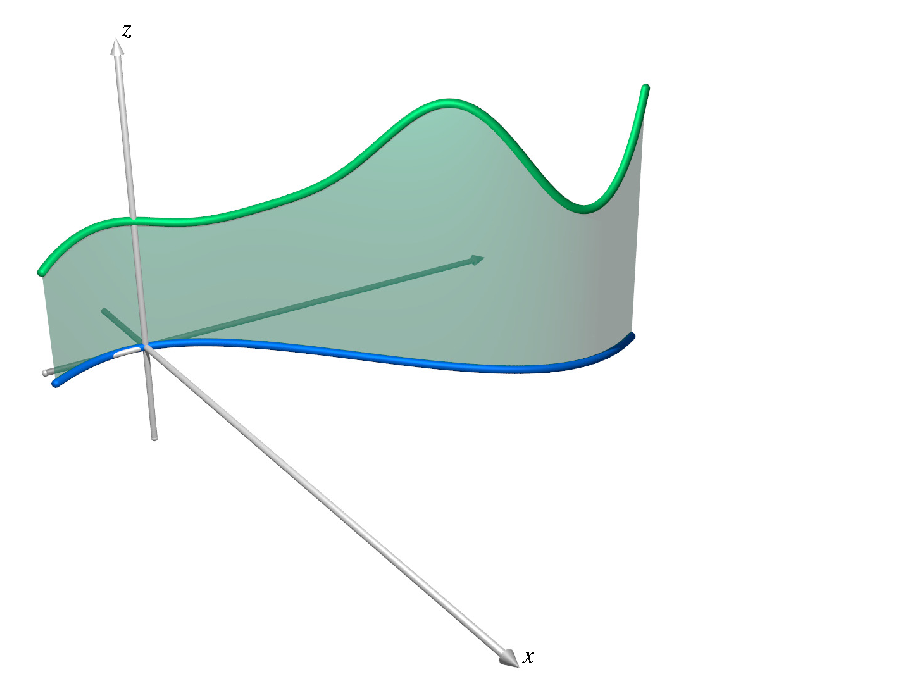
\includegraphics{2-classification/images/cauchycurve.pdf}
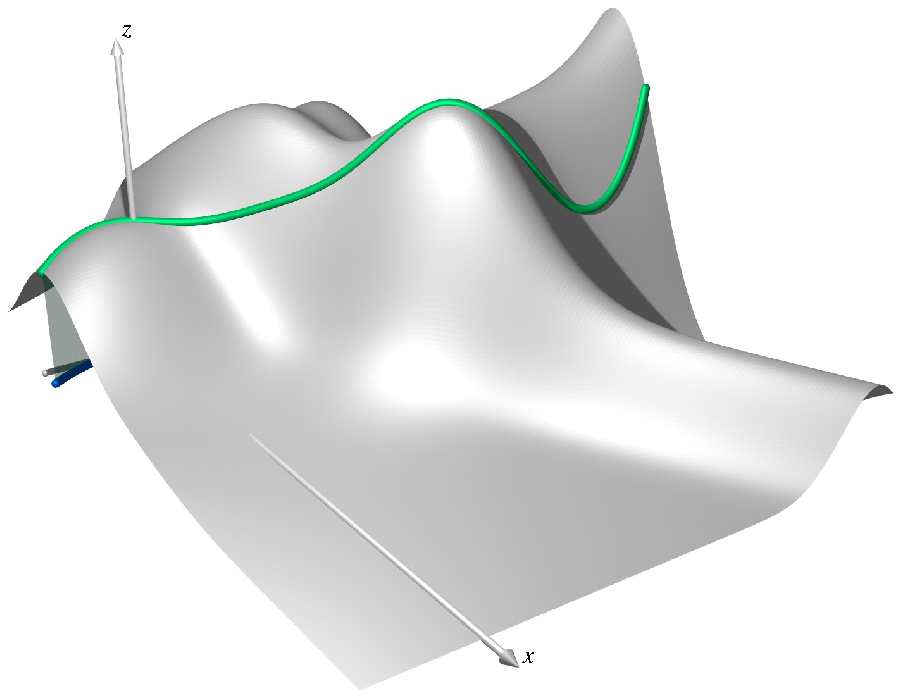
\includegraphics{2-classification/images/cauchy.pdf}%
\caption{Initial curve (top) and surface through the curve (bottom)
\label{cauchy:curve}}
\end{figure}
In general the boundary of a domain is more complicated than just 
a coordinate axis.
Fixing values along the $y$-axis means requesting that the solution
surface contains a curve that projects to the $y$ axis.
A parametrization of the curve would be $y\mapsto (0,y,g(y))$.

The generalization of this idea is the Cauchy problem:

\begin{problem}[Cauchy Problem]
Let $\gamma$ bi a curve in space and 
$F(x,y,u,\partial_xu,\partial_yu)=0$ a partial differential equation.
A function $u(x,y)$ is a solution of the Cauchy problem with initial
curve $\gamma$ if the graph of $u$ contains $\gamma$.
\end{problem}

For each point on the boundary, we can choose a coordinate system such
that the $y$-direction is tangential to the boundary while the $x$-axis
is normal on the boundary.
Then the derivatives we may specify in addition to the boundary
values is just the derivative with respect to $x$.
This derivative is just a directional derivative in a direction normal
to the boundary, we write it
\[
\frac{\partial u}{\partial n}
\]
and call it the normal derivative.
With the choice of coordinate system as describe above, the normal
derivative can be computed using the formula
\[
\frac{\partial u}{\partial n}
=\frac{\partial u}{\partial x}.
\]

If $n$ is the normal vector of a curve ($n=2$) or a surface ($n=3$),
on which boundary conditions are prescribed, then the normal derivative
can be computed using the directional derivative:
\[
\frac{\partial u}{\partial n}=D_nu = n\cdot \operatorname{grad} u.
\]
(See definition~\ref{definition:normal-derivative})

\subsection{General boundary value problem
\label{klassifikation:allgemeines-randwertproblem}}
For partial differential equations the topology of the domain has much
greater influence on the solvability than with ordinary differential
equations, where the topology of the domain is exceedingly simple.
The Cauchy problem discussed in the preceding sections helps us understand
what types of boundary conditions are meaningful.
We have seen that in general, boundary conditions are of the following types:
\begin{itemize}
\item
Values along the boundary of the domain in the form
\[
u(x)=g(x)\quad \forall x\in\partial G\subset \mathbb R^n.
\]
These are called {\em Dirichlet} boundary conditions.
\item
Values of the normal derivative along the boundary, written as
\[
\frac{\partial u}{\partial n}(x)=h(x)\quad\forall x\in\partial G\subset \mathbb R^n.
\]
These are {\em Neumann} boundary conditions.
\item
Linear combinations of values and normal derivatives along the 
bounary.
\end{itemize}
A nice example for mixed boundary conditions is the wave equation of
a vibrating string.
For $t=0$ we specify initial values and initial $t$-derivatives which happen
to be normal derivatives.
These normal derivatives are not needed on the two ends of the interval
for $t>0$.
So we find two types boundary conditions: boundary values along the complete
boundary and normal derivatives times the characteristic function of
the bottom boundary.

Unfortunately, this is not enough to decide which boundary conditions are needed
to fix the solution of the equation.
For this a more in depth theory is required.
This is in stark contrast to the situation for ordinary differential
equations where the Picard-Iteration method guarantees existence and
uniqueness of solutions under very mild conditions on the differential
equation.
We tackle this difficult problem for different types of differential
equations in the following chapters.
But first we must define what it means to have a solution of a partial
differential equation.
